\documentclass[11pt,a4paper]{article}

\usepackage[margin=.6in]{geometry}
\usepackage{graphicx}
\usepackage{booktabs}
\usepackage{hyperref}
\usepackage{listings}
\usepackage{xcolor}
\usepackage{subcaption}
\usepackage[bottom]{footmisc}
\usepackage{cleveref}

\crefformat{section}{\S#2#1#3}
\crefformat{subsection}{\S#2#1#3}
\crefformat{subsubsection}{\S#2#1#3}
\crefformat{figure}{#2Figure~#1#3}
\crefformat{footnote}{#2\footnotemark[#1]#3}
\crefformat{table}{#2Table~#1#3}
\crefformat{equation}{#2Equation~#1#3}

\title{Characterizing Network Traffic with Programmable Dataplanes}
\author{Giuseppe Capasso}
\date{\today}

\begin{document}

\maketitle

\section*{LLM Usage}
LLMs have been used to generate part of the code of this assignment and as a general Python documentation
search engine. In particular:

\begin{itemize}
    \item Distribution fitting: LLM helped when fitting the bimodal creating the code to adapt the distribution left peak and right peak;
    \item \textit{controller.py}: LLM generated the function to retrieve the register using \textit{thrift}
        interface from the CLI.
    \item P4: LLM helped me in defining the flow tracking using the "hash" function and in adapting the code from p4 tutorial.
    \item Plotting: LLM generated part of the code to visualize logarithmic durations and fix the "zero-duration" bug, avoid $\log(0)$
\end{itemize}

LLMs have not been used to write this document.

\section{Introduction}
In this assignment, I analyzed a $15$ minutes long network capture with two different methodologies:

\begin{itemize}
    \item \textbf{Software based characterization}: I analyzed the data coming from the network \textit{simply} converting the original \texttt{PCAP} in a \texttt{CSV};
    \item \textbf{In-Network based analysis}: I extracted the feature directly on the data-plane using a \textit{P4} program and \textit{bmv2} switch;
\end{itemize}

This document contains a comparison between both methodologies, for further technical details refer to the other artifacts of the repository\footnote{Repository is publicly available on Github at \url{https://github.com/alarmfox/imdea-assignement}}.

The rest of document is organized as follows. \cref{sec:results} discusses the general results from the analysis. \cref{sec:comparison} presents differences between the two methodologies.

\section{Analysis and Results}
\label{sec:results}

In this section, I explain results obtained using the full dataset.

\subsection{Packet-level analysis}
As a packet level feature, I analyzed the packet sizes. The PDF is shown in \cref{fig:pdf-packet-size}. As in classical network environments, packet size is limited by the Maximum Transmission Unit (MTU) which is $1500$. The behaviour is that the most majority of the traffic has either short lived messages (ICMP and other control/signaling protocols) or near to the MTU.

\begin{figure}
    \centering
    \begin{subfigure}{.8\textwidth}
        \centering
        
\includegraphics[width=\textwidth]{../figures/task1/pdf-packet_size.pdf}
        \caption{Packet-size distribution}
        \label{fig:pdf-packet-size}
    \end{subfigure}\hfill
    \begin{subfigure}{.8\textwidth}
        \centering
        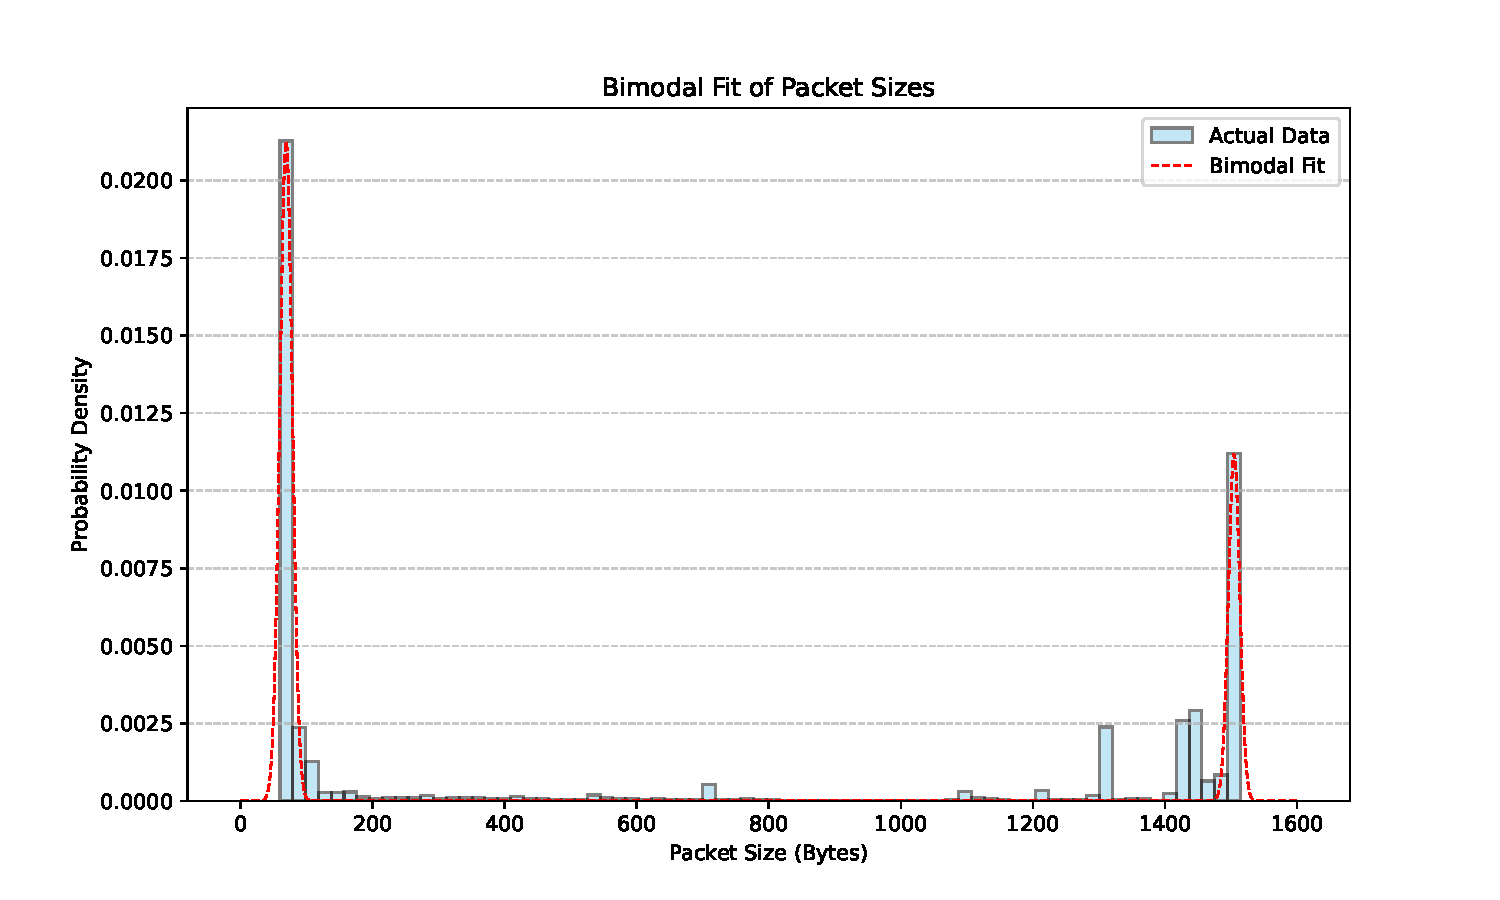
\includegraphics[width=\textwidth]{../figures/task1/bimodalfit-packet-size.pdf}
        \caption{Packet-size distribution}
        \label{fig:pdf-packet-size-fitting}
    \end{subfigure}\hfill
    \caption{Analysis of network packet sizes: raw data vs. statistical fit.}
\end{figure}

\paragraph{Distribution fitting} Looking at the distribution in \cref{fig:pdf-packet-size}, I can clearly fit a \textbf{bimodal} distribution\footnote{In this simple case, the bi-modal distribution has been generated as the sum of two normal distributions.}. I estimated parameter using \textbf{scipy} \texttt{curve\_fit}. The result of this fitting is shown in \cref{fig:pdf-packet-size-fitting}. The goodness of fit is evaluated using $R^2$ (\cref{eq:rsquared}) and $RMSE$ (\cref{eq:rmse}).

$0 \leq R^2 \geq 1$. A high $R^2$ tells we have a good fit. On the other hand, a low $RMSE$ tells we have a good fit. $RMSE$ is an easy to calculate factor, but it is sensitive when dealing outliers.

\begin{equation}
    \label{eq:rsquared}
    R^2 = 1 - \frac{SS_{res}}{SS_{tot}}
\end{equation}

$\overline{y}$ is the mean of the initial dataset. $y_i$ is a point of the initial dataset. $f_{i}$ is a point of the fitted distribution.

$SS_{res}$ is the sum of square of residual. It indicates how much data fitted in the model differs from the mean value of original data (we take always the sum of squares to remove negative values).
\begin{equation}
    SS_{res} = \sum_{i=1}^n (y_i - f_i)^2
\end{equation}

$SS_{tot}$ is the total sum of squares. It is obtained with the difference between $y_i$ and $\overline{y}$
\begin{equation}
    SST = \sum_{i=1}^n (y_i - \overline{y})^2
\end{equation}

$RMSE$ is the mean distance between predicted data and original data squared:

\begin{equation}
    \label{eq:rmse}
    RMSE = \sqrt{\frac{1}{n}\sum_{i=1}^n (y_i - f_i)^2}
\end{equation}


In this case, $R^2 > 0.9$ so the `curve\_fit` parameters are a good approximation of the initial dataset.

\subsection{Flow-level analysis}
As flow level metrics, I analyzed the flow duration and analyzed TCP and UDP specific characteristics. Looking at flow duration distribution, \cref{fig:flow-duration-distribution} shows that the vast majority of flows (both TCP and UDP) are short lived (many of them have $0$ second duration).

\begin{figure}
    \centering
    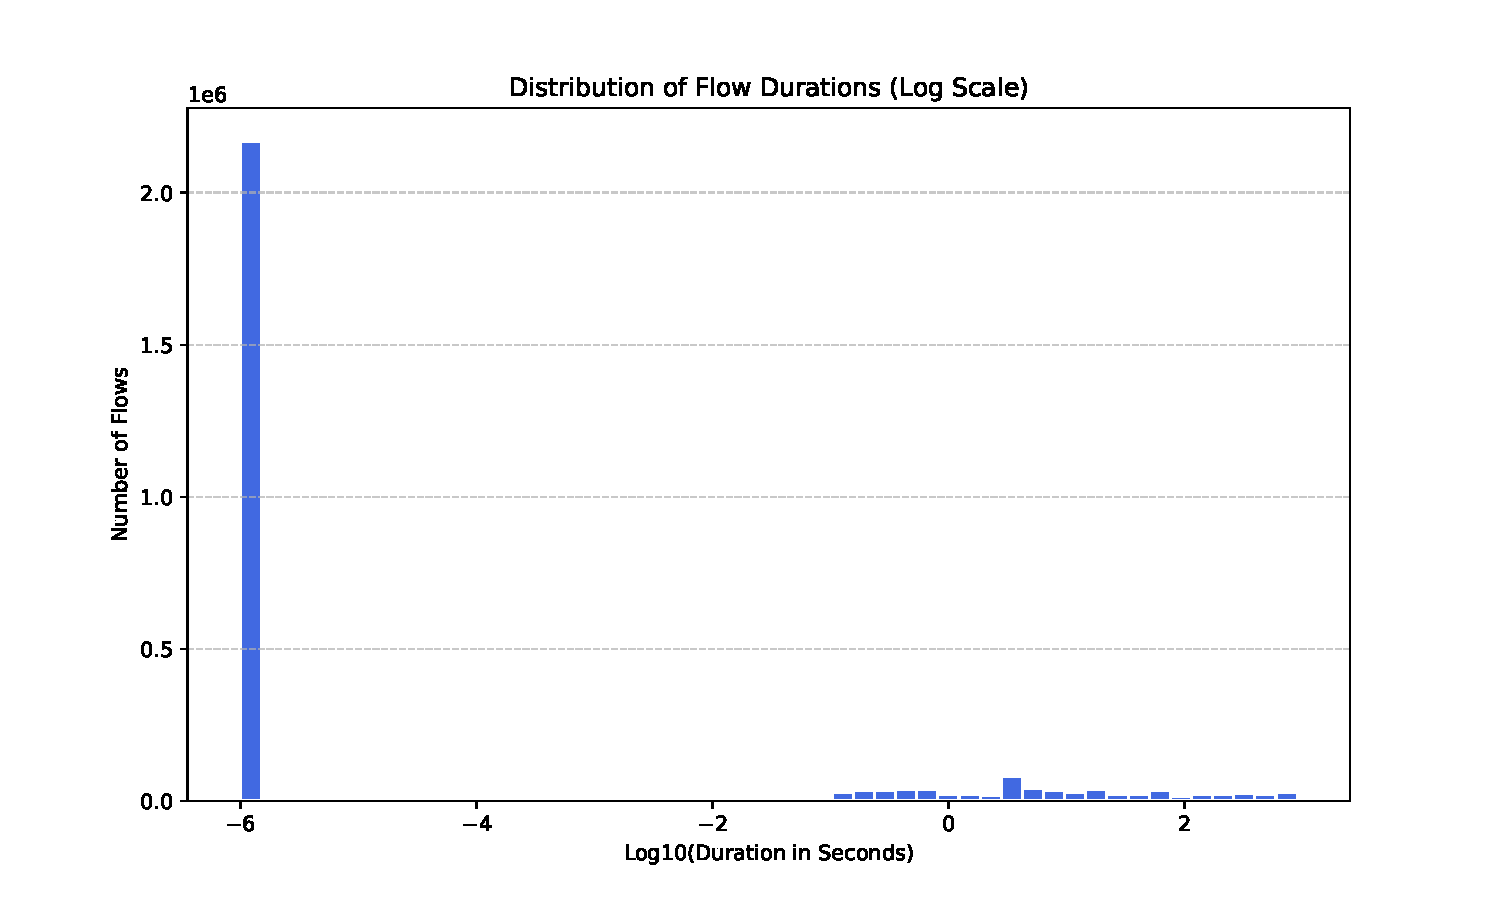
\includegraphics[width=0.8\textwidth]{../figures/task1/distribution-flow-durations-all.pdf}
    \caption{Log-scale distribution of flow durations.}
    \label{fig:flow-duration-distribution}
\end{figure}

To further understand the nature of this phenomenon, I classify the flows by protocol (\cref{fig:proto-byflow}) and by data exchanged (\cref{fig:proto-bybytes}). Results tells that:
\begin{itemize}
    \item $~44\%$ of the traffic is ICMP and it exchanges less than $10\%$ of data;
    \item $~31\%$ of the traffic is TCP and it exchanges more than $80\%$ of data;
    \item $~19\%$ of the traffic is UDP and it exchanges $~6\%$ of data.
\end{itemize}

\begin{figure}
    \centering
    \begin{subfigure}{.5\textwidth}
        \centering
        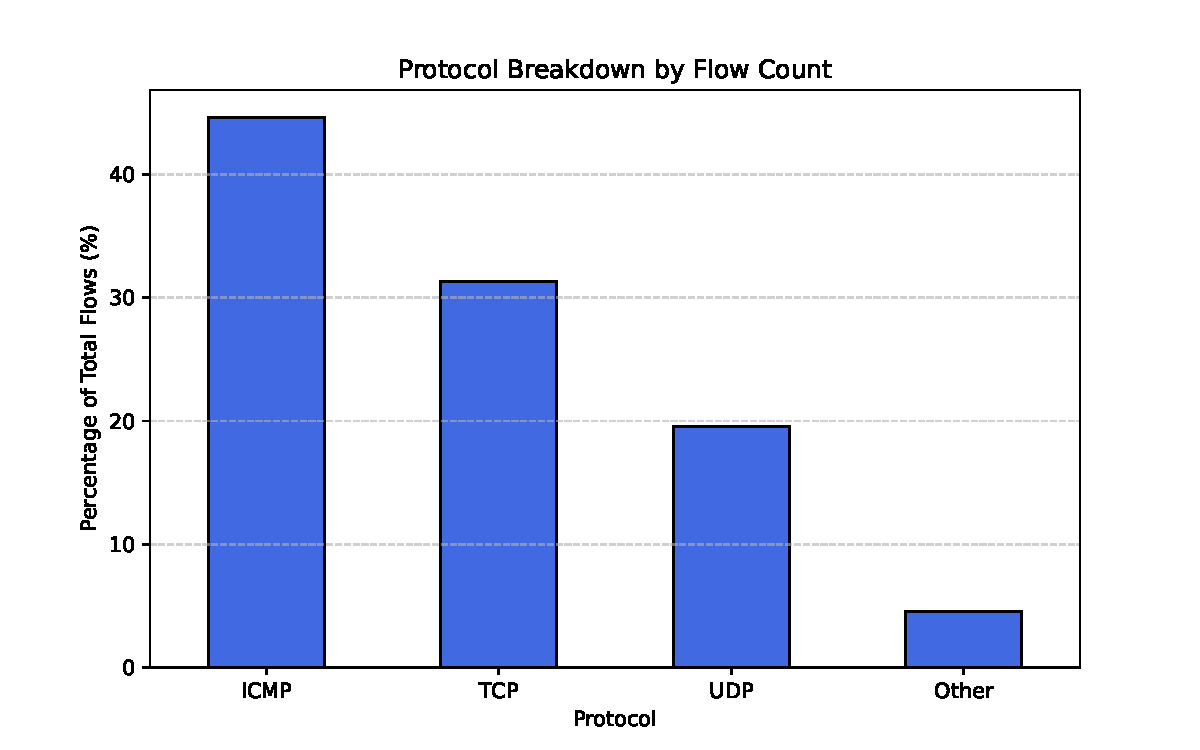
\includegraphics[width=\textwidth]{../figures/task1/proto-byflow.pdf}
        \caption{Flow classification by protocol}
        \label{fig:proto-byflow}
    \end{subfigure}\hfill
    \begin{subfigure}{.5\textwidth}
        \centering
        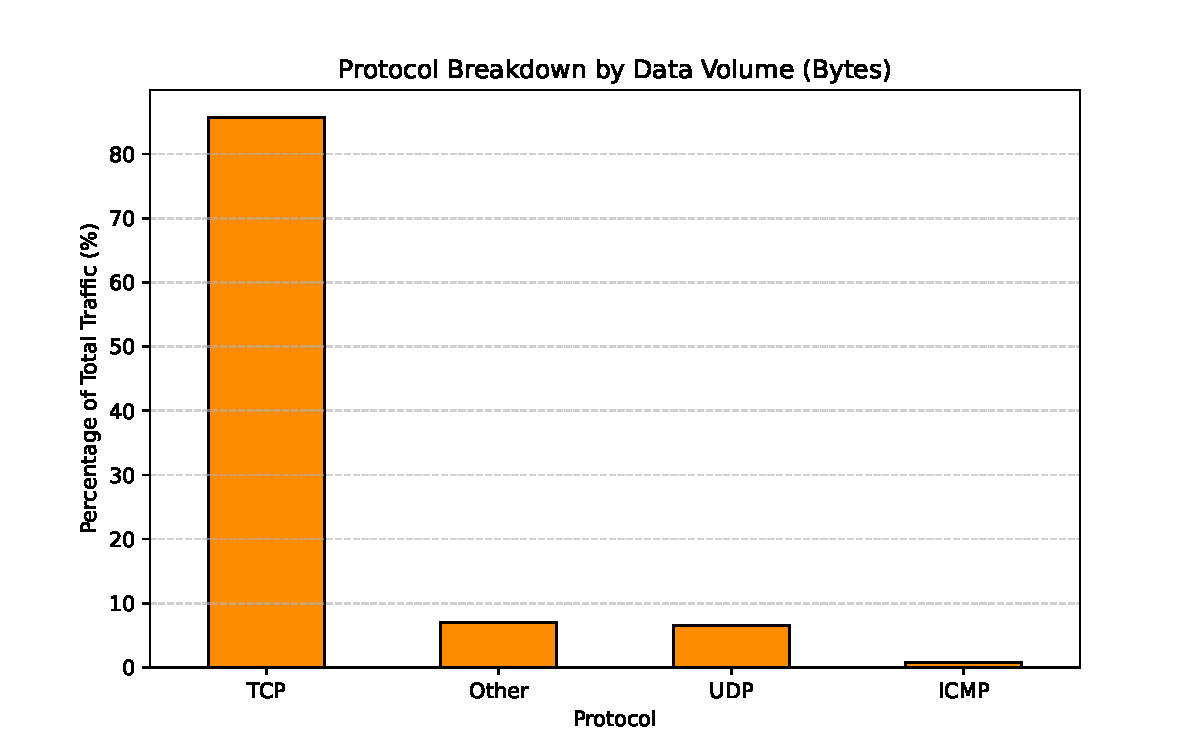
\includegraphics[width=\textwidth]{../figures/task1/proto-bybytes.pdf}
        \caption{Flow classification by bytes exchanged}
        \label{fig:proto-bybytes}
    \end{subfigure}\hfill
    \caption{Flow classification by protocol and bytes sent}
\end{figure}

Removing the ICMP, noise it is clear that TCP traffic with low duration is \textit{strange}. So I analyzed the TCP flows with less than $4$ packets (as it indicates that the handshaske was not completed). \cref{fig:tcp-durations-flow} shows that the low durations TCP connections are the ones that do not complete handshake. \cref{fig:tcp-broken-perc} shows that $~51\%$ of TCP connections are not valid. This is an indication that there might be a network scan going on.

\begin{figure}
    \centering
    \begin{subfigure}{.5\textwidth}
        \centering
        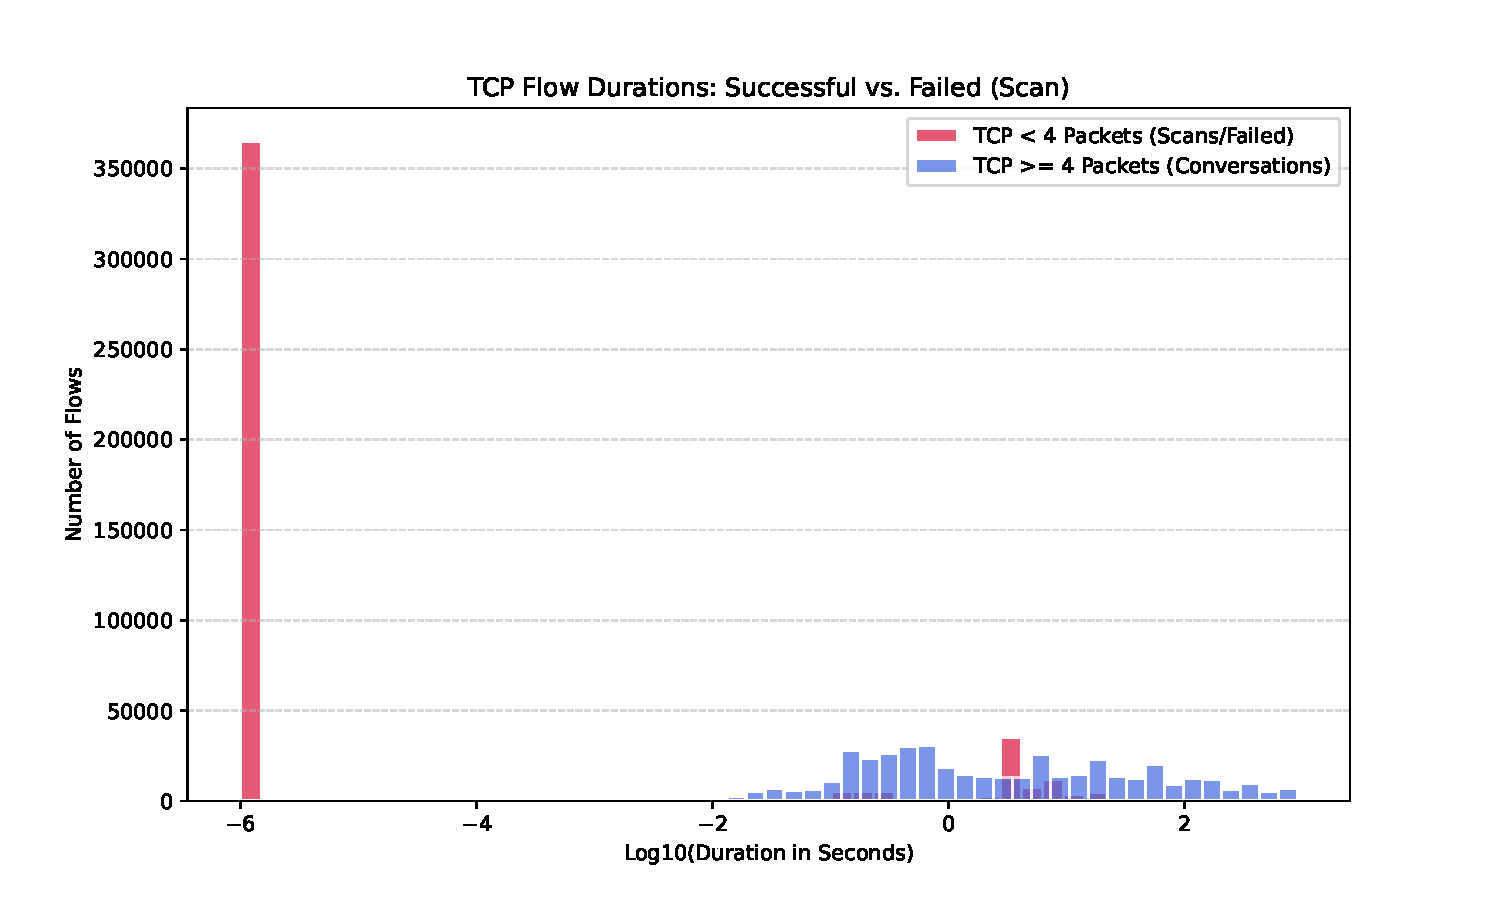
\includegraphics[width=\textwidth]{../figures/task1/tcp-durations-broken-vs-ok.pdf}
        \caption{TCP durations: $packet \geq 4$ vs $packet < 4$}
        \label{fig:tcp-durations-flow}
    \end{subfigure}\hfill
    \begin{subfigure}{.5\textwidth}
        \centering
        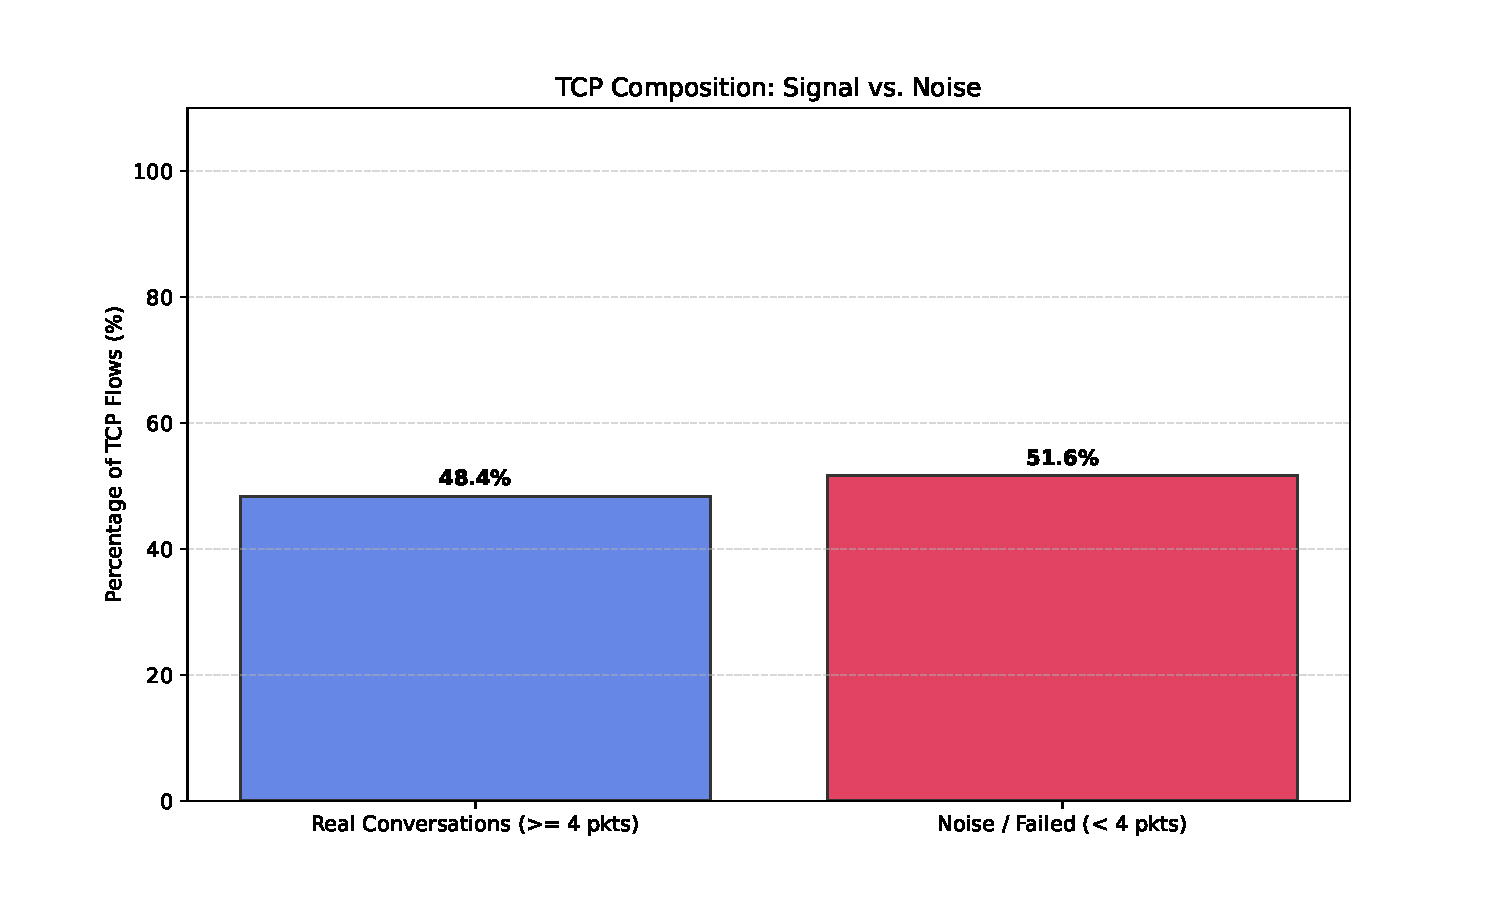
\includegraphics[width=\textwidth]{../figures/task1/tcp-perc-broken-vs-ok.pdf}
        \caption{Percentage of TCP flows with $packet \geq 4$ vs $packet < 4$}
        \label{fig:tcp-broken-perc}
    \end{subfigure}\hfill
    \caption{TCP flow analysis: broken handshake vs successful connections}
\end{figure}

I performed a similar analysis on UDP flows. In this case, a zero second UDP flows could mean either a single packet with no answer (eg. a failed DNS query) or a probe. Similarly to TCP, \cref{fig:udp-durations-flow} and \cref{fig:udp-broken-perc} shows that the $~87\%$ of UDP flows have zero duration.

\begin{figure}
    \centering
    \begin{subfigure}{.5\textwidth}
        \centering
        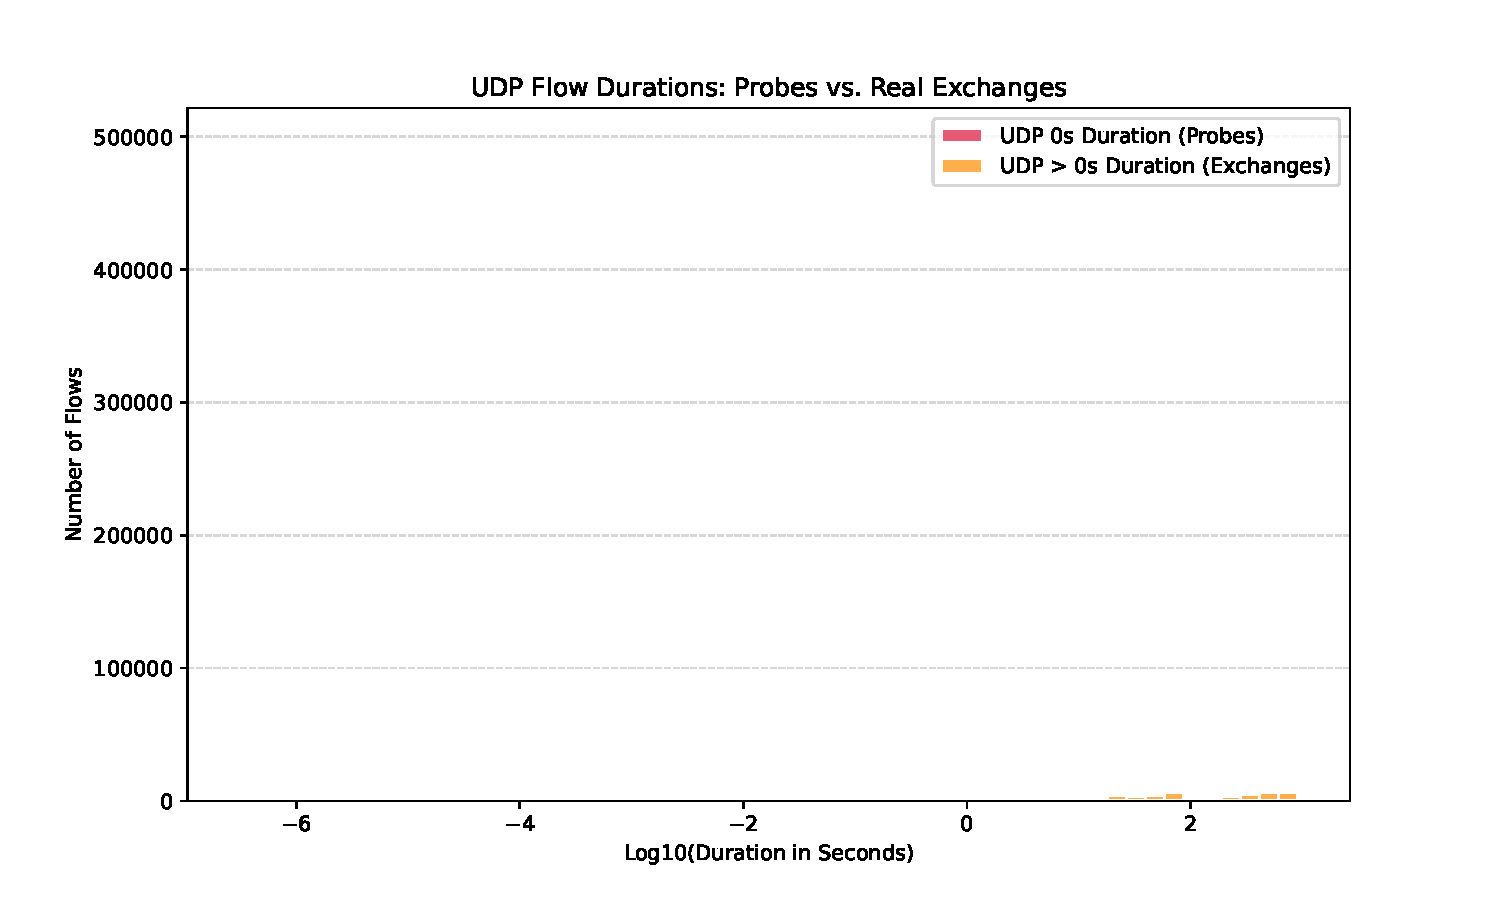
\includegraphics[width=\textwidth]{../figures/task1/udp-durations-zero-vs-real.pdf}
        \caption{UDP flow durations: failed vs success}
        \label{fig:udp-durations-flow}
    \end{subfigure}\hfill
    \begin{subfigure}{.5\textwidth}
        \centering
        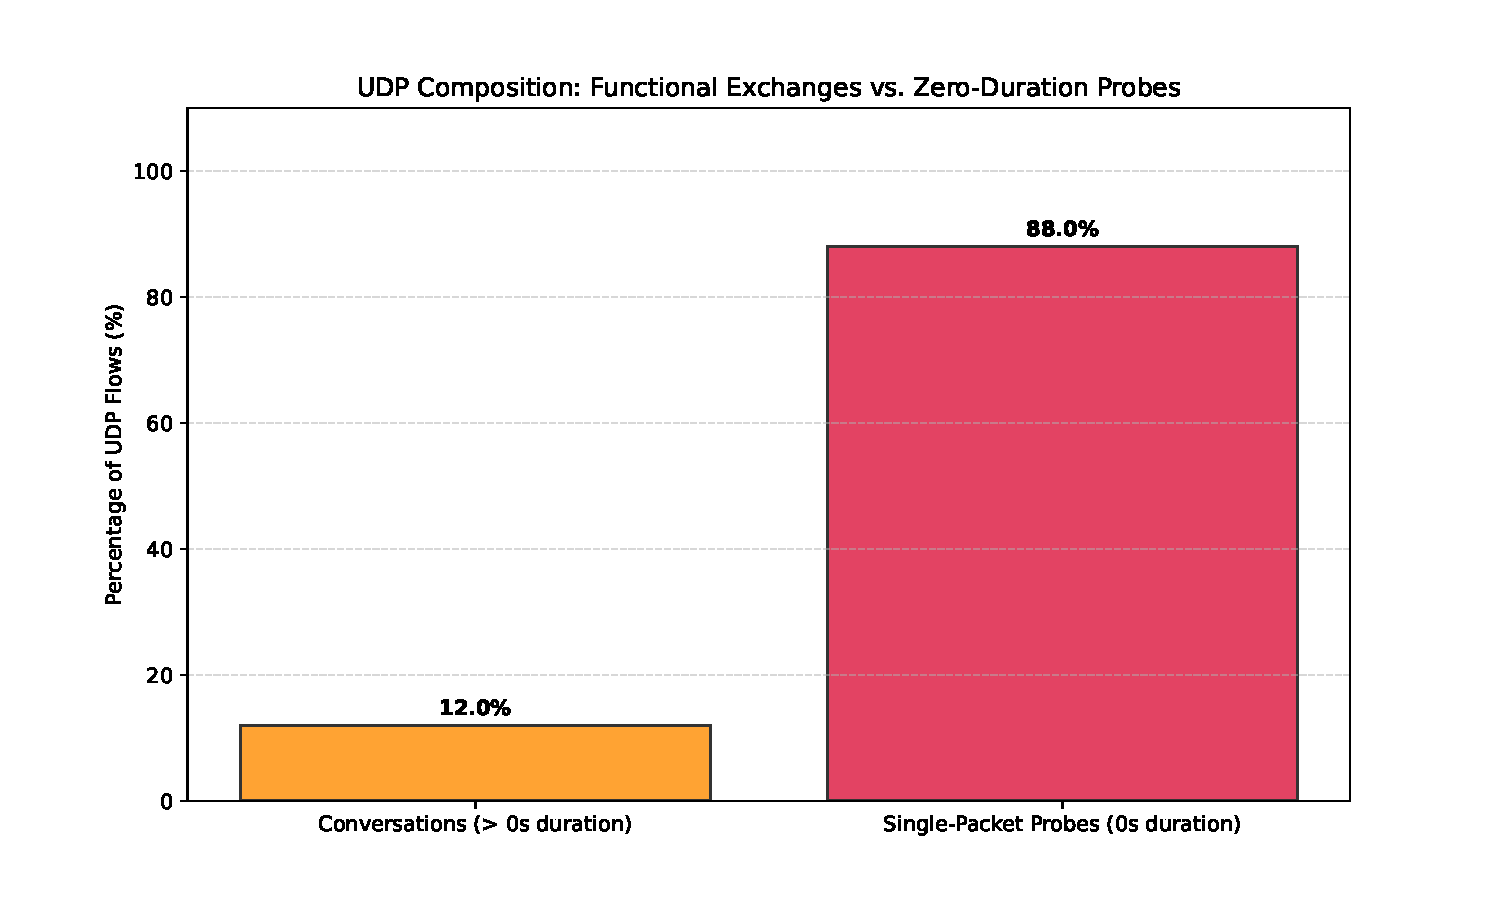
\includegraphics[width=\textwidth]{../figures/task1/udp-perc-zero-vs-real.pdf}
        \caption{Percentage of zero duration flows}
        \label{fig:udp-broken-perc}
    \end{subfigure}\hfill
    \caption{UDP flow analysis: probes/failed vs successful connections}
\end{figure}

Removing the noise from ICMP traffic, invalid TCP and UDP connection, \cref{fig:network-profile} shows the cleaned-up network profile. Most of TCP and UDP connections last from $10-100$

\begin{figure}
    \centering
    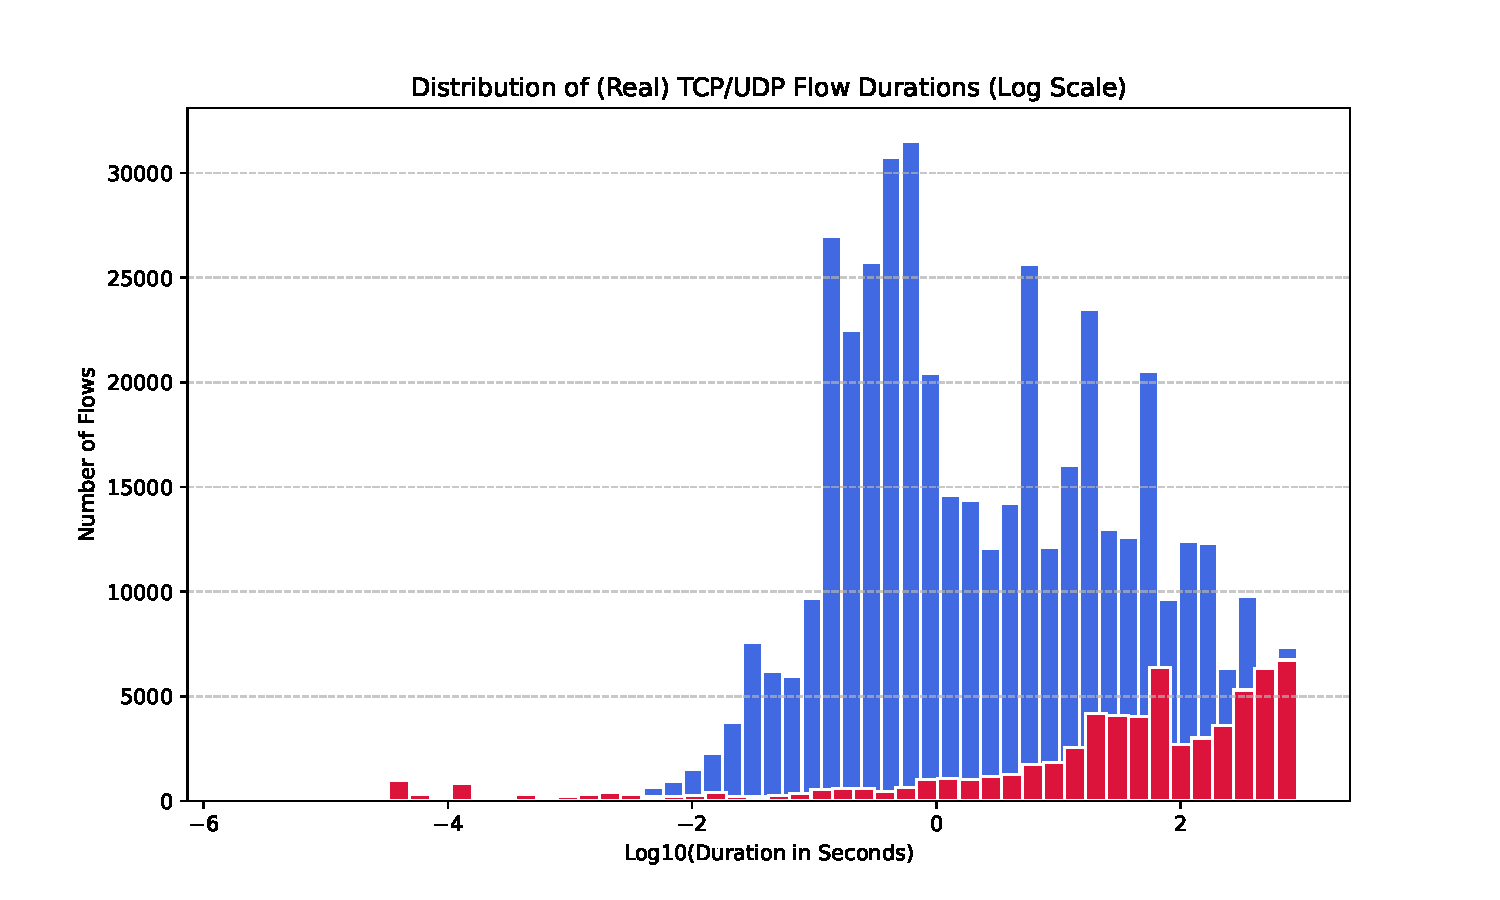
\includegraphics[width=0.8\textwidth]{../figures/task1/distribution-flow-durations-tcpudp.pdf}
    \caption{De-noised network profile}
    \label{fig:network-profile}
\end{figure}

\subsection{Security considerations}
The high volume of ICMP traffic combined with a vast number of incomplete TCP handshakes strongly suggests active network reconnaissance (scanning). The prevalence of zero-second UDP flows further supports this, as they likely represent probes to closed ports. To confirm, Deep Packet Inspection (DPI) or a port-frequency analysis is recommended to identify the specific nature of the UDP and ICMP traffic (e.g., DNS vs. unusual probing).

To identify the source of the potential network scan, I analyzed the traffic profile of individual source IPs\footnote{I know that IP addresses are anonymized, but this analysis leverages the fact that common tools (like `tcpreplay` or `editcap`) use a consistent mapping.
}. The underlying hypothesis is that a network scanner exhibits a highly asymmetric traffic pattern: it initiates a massive number of connections (flows) to probe ports, but transmits virtually no application data.

To test this, I aggregated the data by Source IP (ip.src)(\cref{fig:top10-ip-flowcount} and \cref{fig:top10-ip-data}) to calculate both the total flow count and the total bytes transmitted per host. By comparing the top 10 most active IPs by flow count against the top 10 IPs by data volume, we can isolate the scanner. Any IP that dominates the flow count but is entirely absent from the top data exchangers is confirmed to be exhibiting scanning behavior.

\begin{figure}
    \centering
    \begin{subfigure}{.5\textwidth}
        \centering
        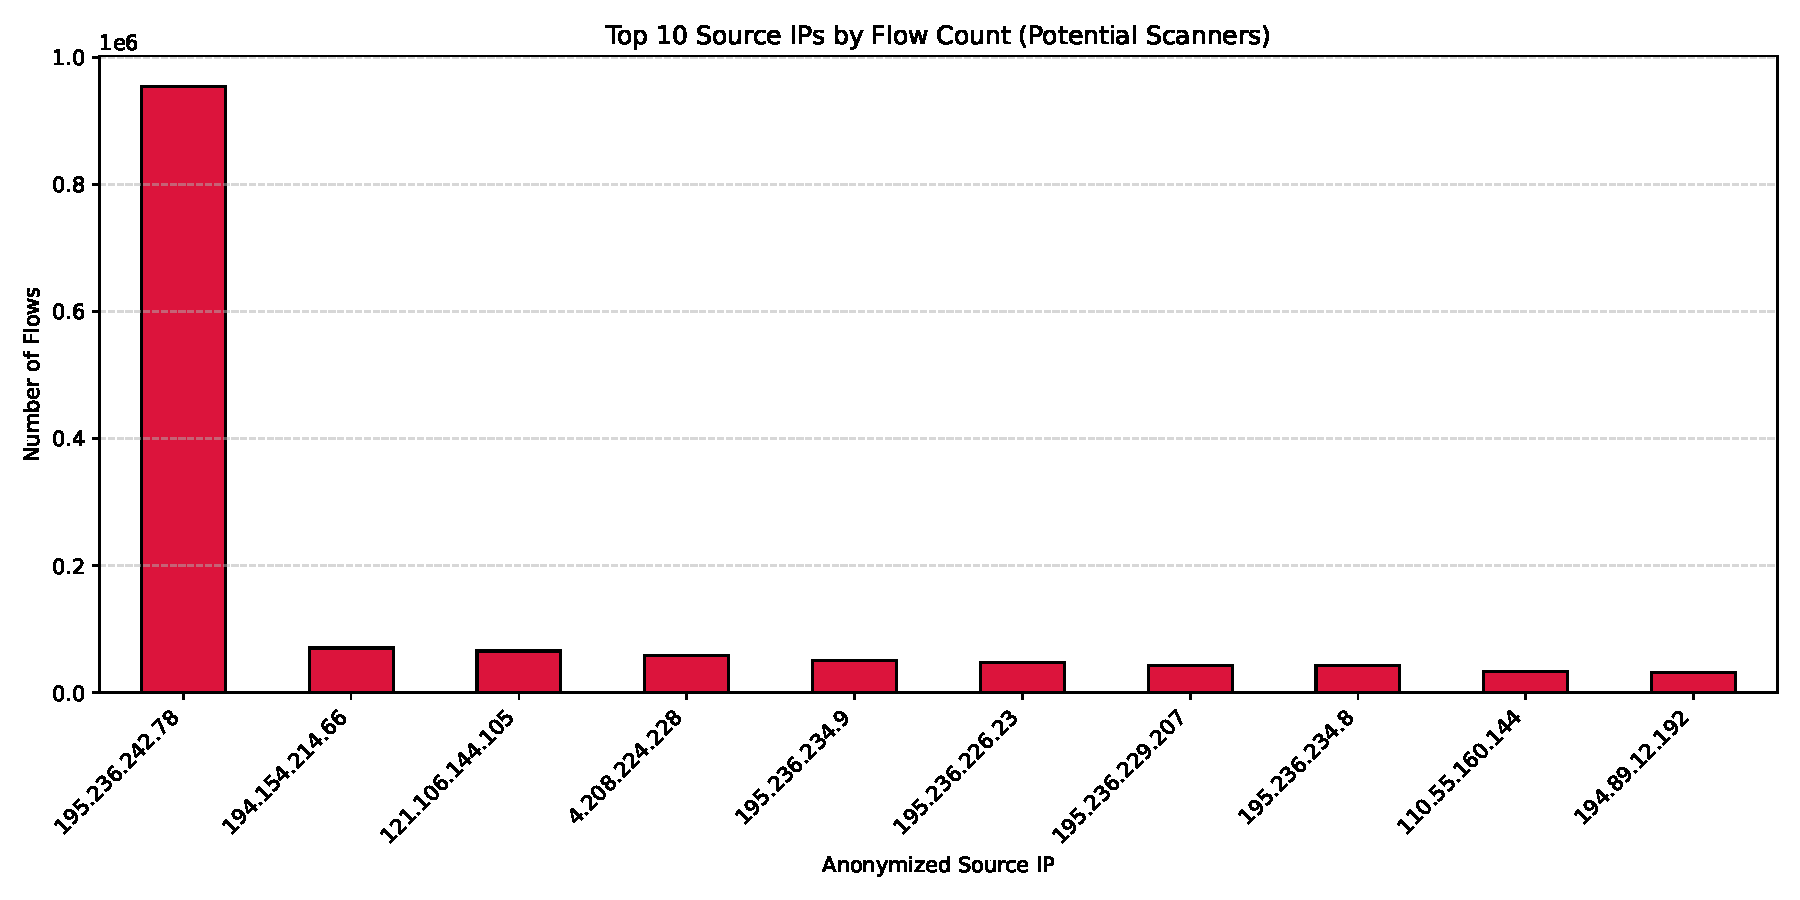
\includegraphics[width=\textwidth]{../figures/task1/top10-srcip-flowcount.pdf}
        \caption{Top 10 IP to initiate flows}
        \label{fig:top10-ip-flowcount}
    \end{subfigure}\hfill
    \begin{subfigure}{.5\textwidth}
        \centering
        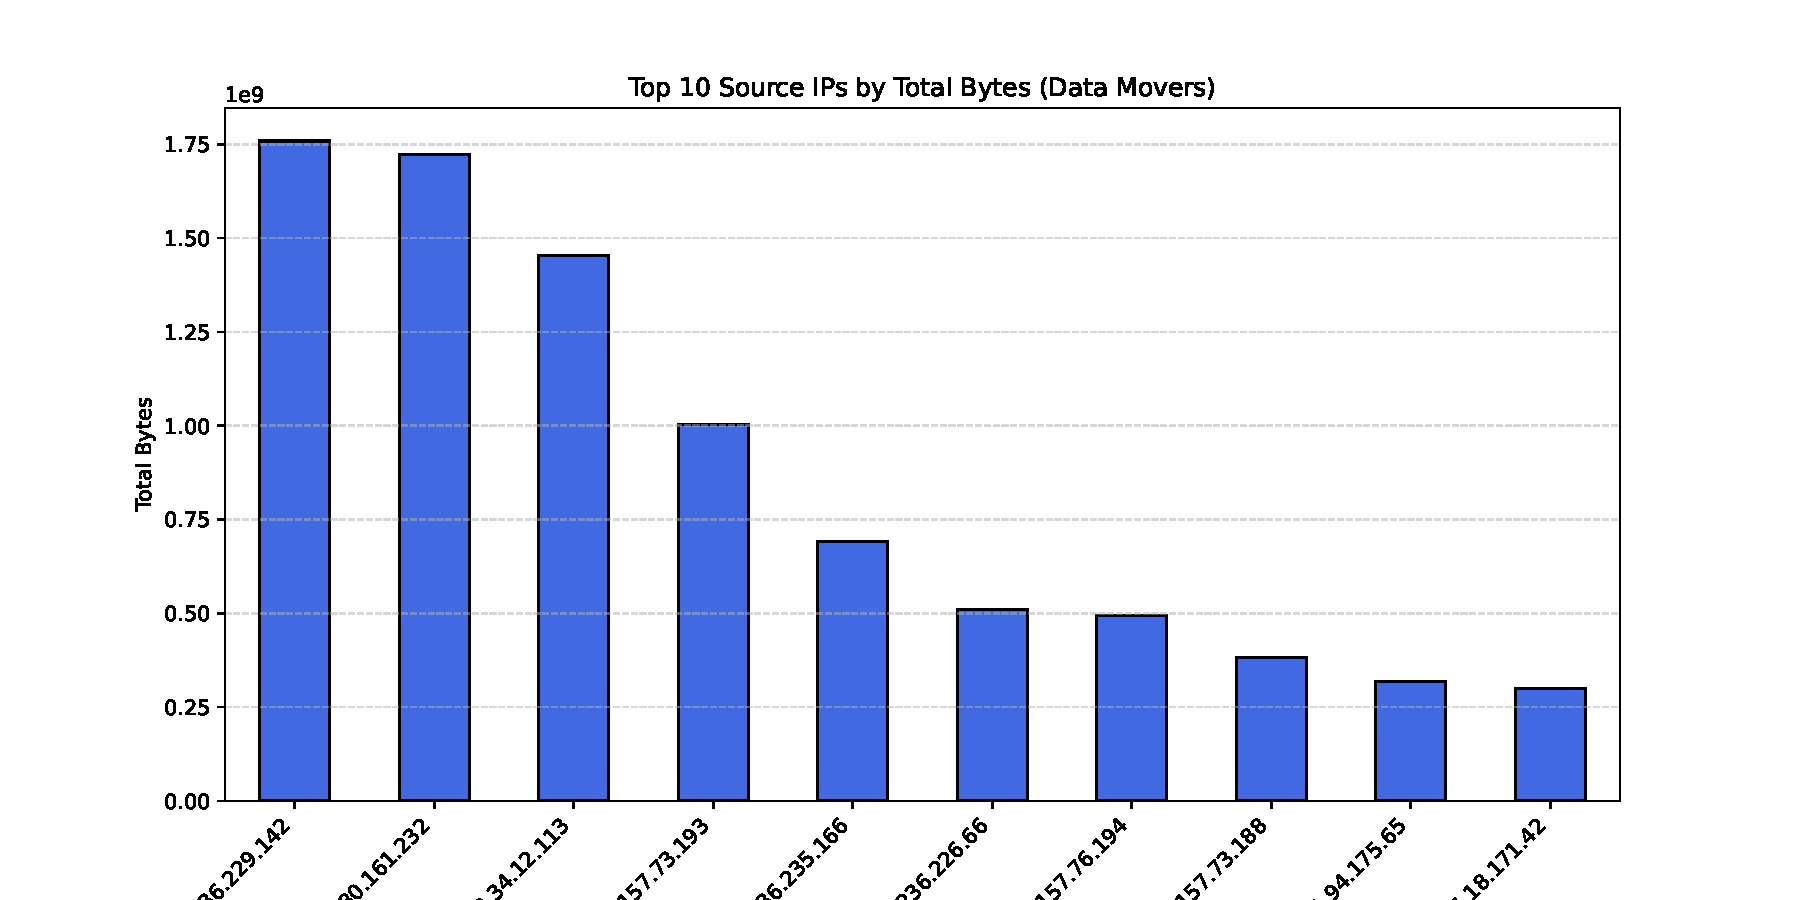
\includegraphics[width=\textwidth]{../figures/task1/top10-srcip-datasent.pdf}
        \caption{Top 10 IP by total bytes}
        \label{fig:top10-ip-data}
    \end{subfigure}\hfill
    \caption{Scanner IP detection.}
\end{figure}

\section{Methodologies comparison: Software-Based vs In-Network Classification}
\label{sec:comparison}
The analysis performed using the \textbf{bmv2} virtual switch extract features at line rate. Results are comparable to what has been shown \cref{sec:results}\footnote{Due to performance limitation of the \textit{bmv2} switch, \textit{tcpreplay} shows a $~5\%$ packet loss.}.

For example, \cref{fig:packetsize-task1-task-2} shows how results are similar to both methodologies. \cref{fig:sw-flow-duration} and \cref{fig:bvm2-flow-duration} also show comparable results between different methodologies.

\begin{figure}
    \centering
    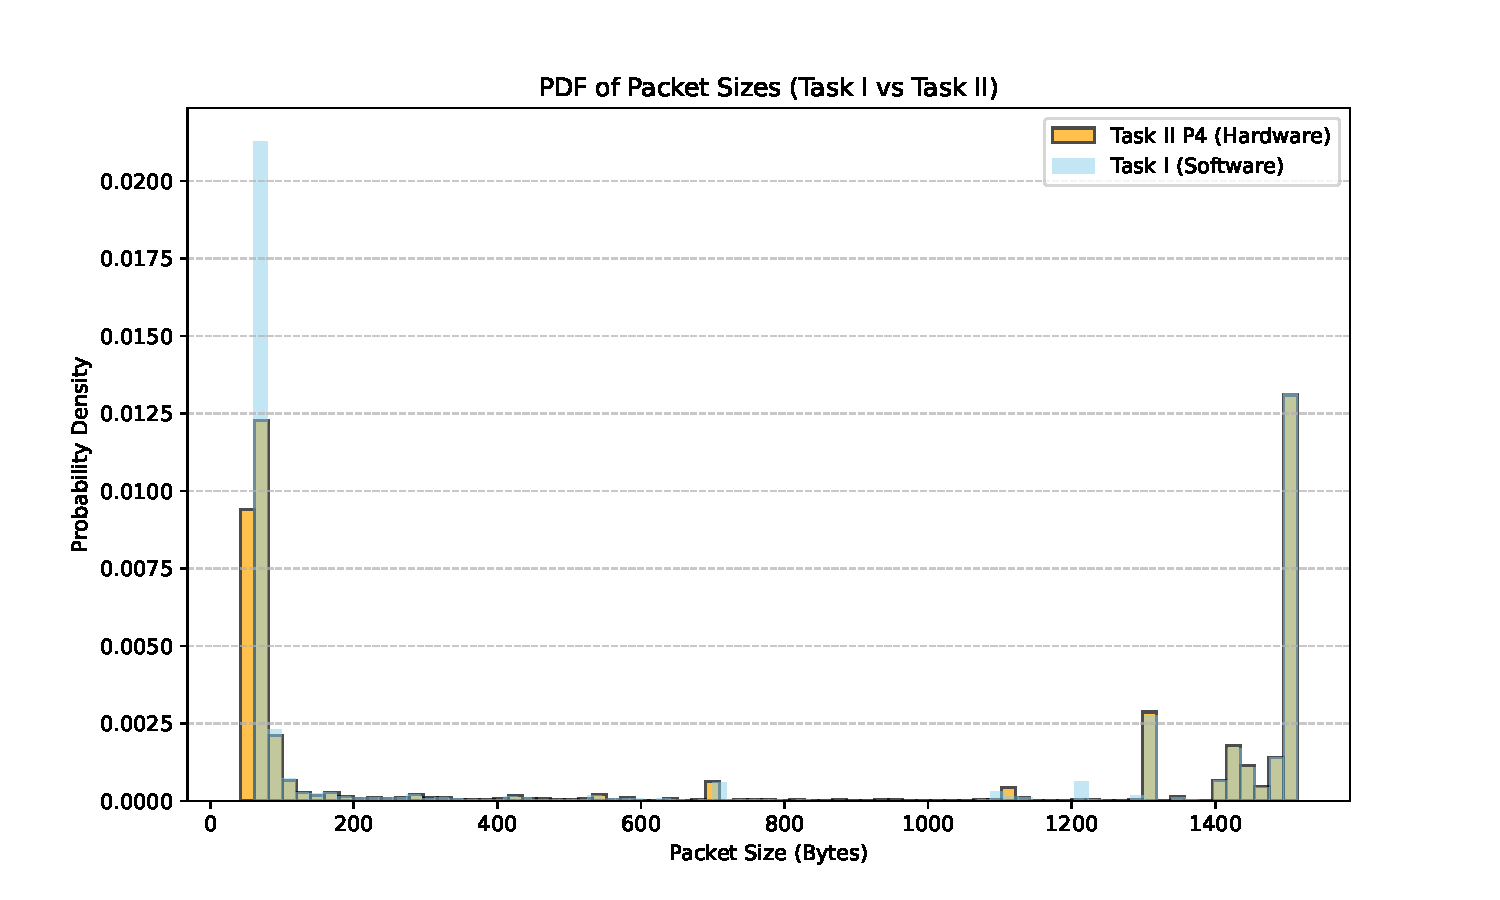
\includegraphics[width=0.8\textwidth]{../figures/task2/pdf-packetsize-task1-task2.pdf}
    \caption{Packet size distribution comparison between Task 1 and Task 2}
    \label{fig:packetsize-task1-task-2}
\end{figure}


\begin{figure}
    \centering
    \begin{subfigure}{.5\textwidth}
        \centering
        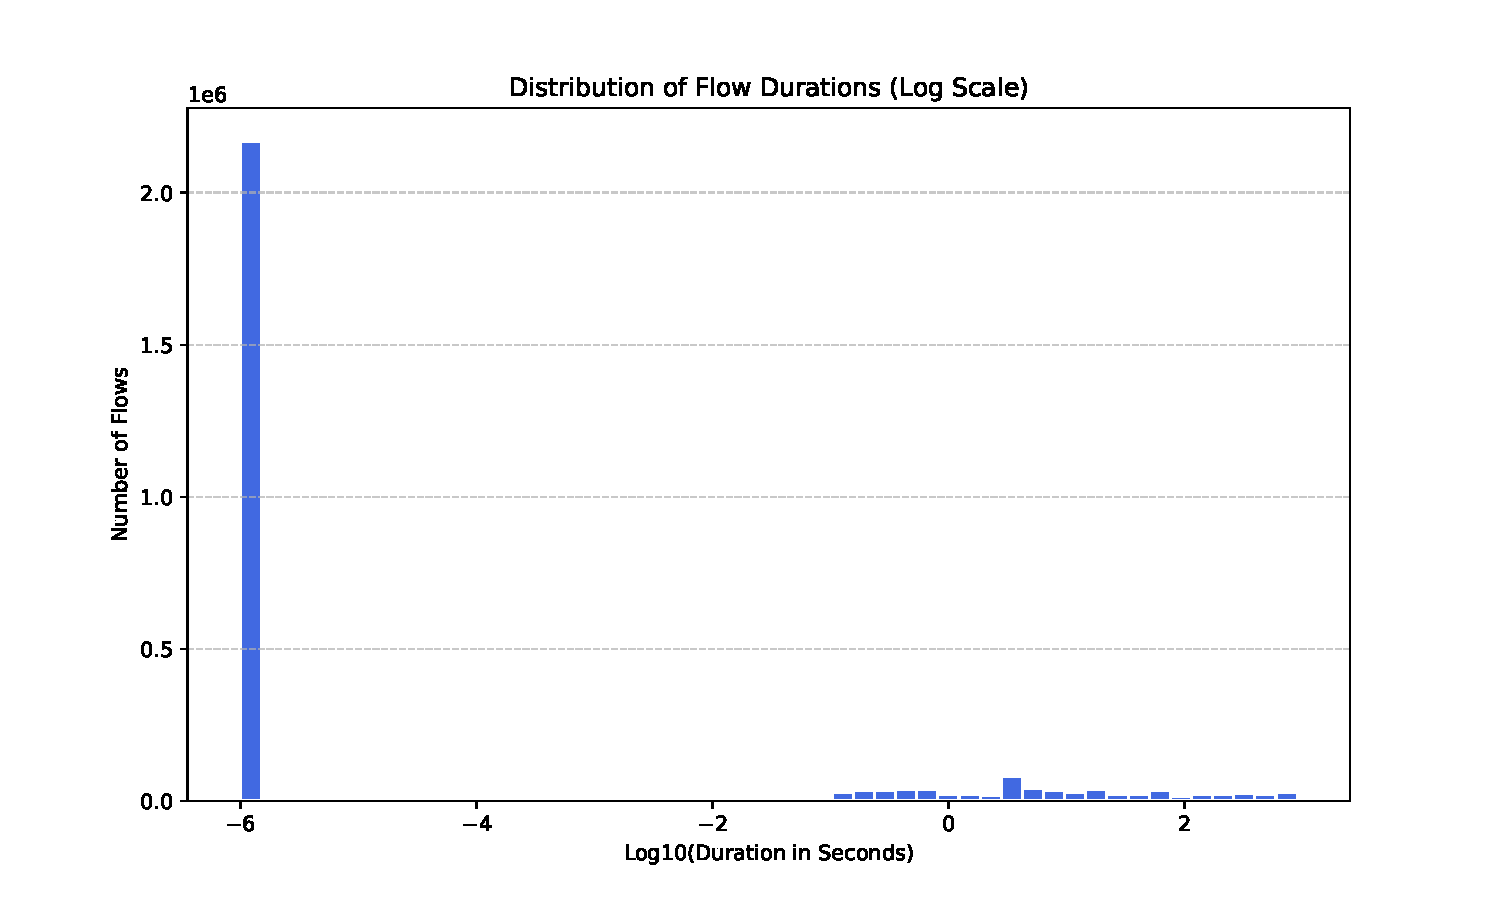
\includegraphics[width=\textwidth]{../figures/task1/distribution-flow-durations-all.pdf}
        \caption{\textit{Software-based} methodology}
        \label{fig:sw-flow-duration}
    \end{subfigure}\hfill
    \begin{subfigure}{.5\textwidth}
        \centering
        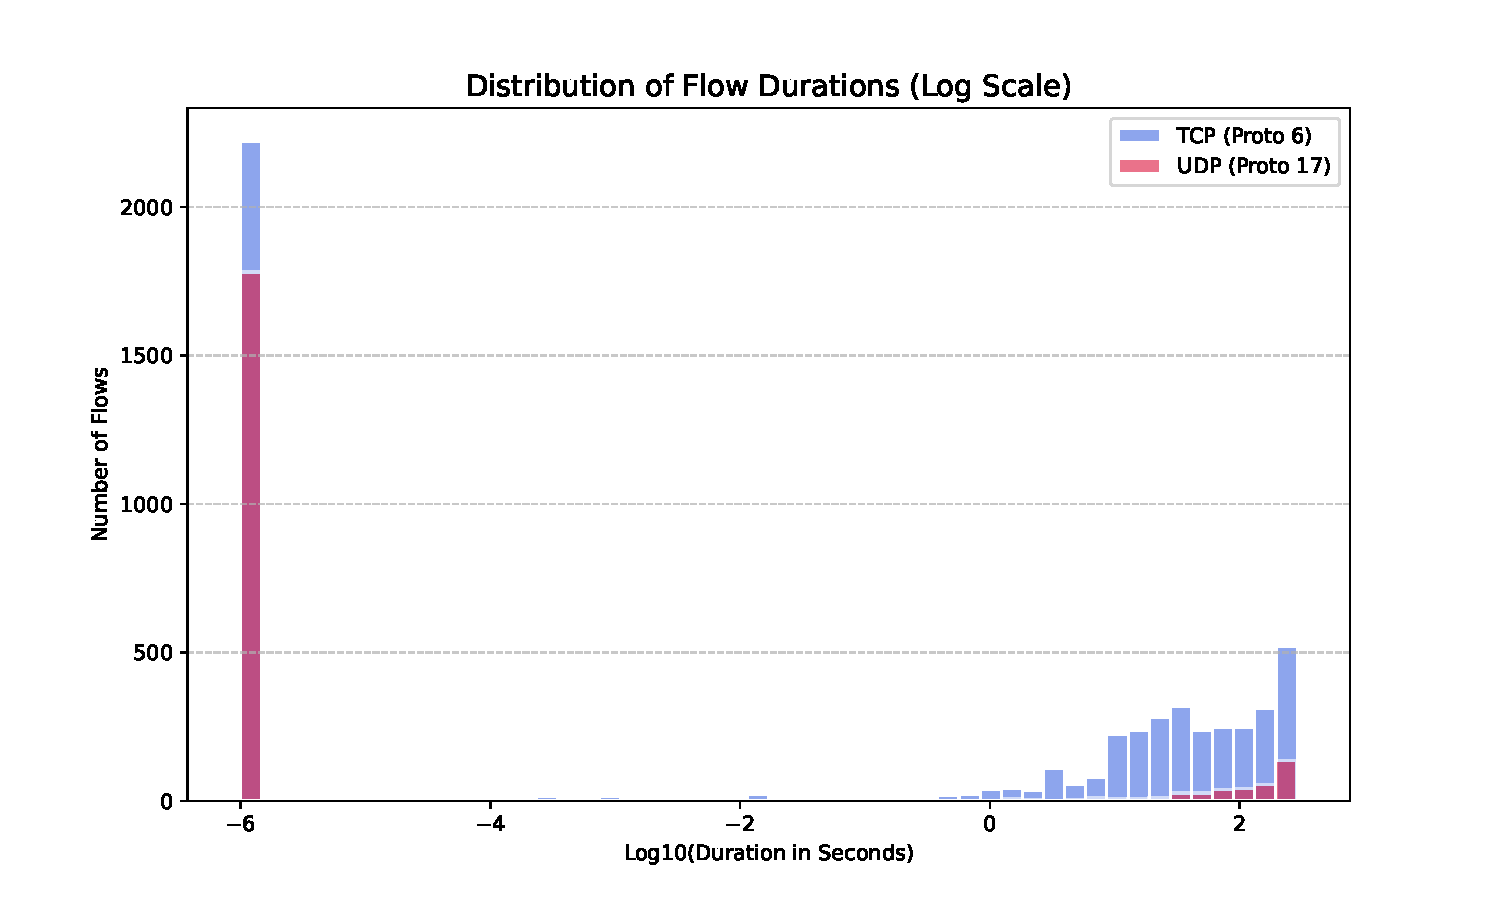
\includegraphics[width=\textwidth]{../figures/task2/distribution-flow-durations.pdf}
        \caption{\textit{In-network} methodology}
        \label{fig:bvm2-flow-duration}
    \end{subfigure}\hfill
    \caption{Comparison between flow duration using both methodologies}
\end{figure}

A comparison between the two methodologies is summarized in \cref{tab:methodology_comparison}.

\paragraph{Throughput and Storage Efficiency}
Moving from software analysis to in-network classification completely changes how we handle performance and data. When relying on Python and PCAP files, the system hits a bottleneck quickly. Parsing times and I/O constraints simply don't scale well as traffic spikes. On top of that, capturing full payloads for deep packet inspection creates a massive storage burden, generating gigabytes of raw data in minutes. The P4 approach solves this by operating directly at line rate, letting the hardware push terabit speeds. Because it only looks at headers and extracts metadata summaries, it shrinks those gigabytes of traffic down into tiny, manageable CSV files.

\paragraph{Detection Latency and Actionability}
The Python approach is ultimately a post-mortem tool. It’s great for forensics, but by the time we analyze the report, the attack is already over. The in-network method, on the other hand, processes packets live. Since the switch extracts features while the traffic is actively flowing, it's possible to build automated feedback loops. If a port scanner appears, the controller can instantly deploy a dynamic firewall rule to drop the packets.

\paragraph{Programmability and Architectural Constraints}
Software provides us with almost total freedom; we can readily utilize floating-point mathematics, comprehensive statistical libraries, and stateful objects to track network behavior. The P4 data plane offers none of these advantages. It is inherently rigid and fundamentally stateless. To maintain line-rate speeds, programmable switches are constrained by limited ALUs and strict pipeline stages, meaning that complex mathematical operations must be significantly simplified. Even tracking a standard multi-packet connection requires us to manually construct state using hardware registers.

\begin{table}
    \centering
    \small
    \caption{Comparison of Software-Based (Post-Mortem) and In-Network (P4) Classification}
    \label{tab:methodology_comparison}
    \begin{tabular}{@{} l p{5cm} p{5cm} @{}}
        \toprule
        \textbf{Feature} & \textbf{Software-Based (Python/PCAP)} & \textbf{In-Network (P4/BMv2)} \\
        \midrule
        \textbf{Timing} & Post-mortem (analysis after attack). & Real-time (during packet processing). \\
        \textbf{Storage} & High: Gigabytes of raw PCAP files. & Minimal: Tiny CSVs of aggregated stats. \\
        \textbf{Throughput} & Bottlenecked by I/O and parsing time. & Line rate (capable of Terabit speeds). \\
        \textbf{Flexibility} & High: Complex libraries, floating point. & Low: Limited by ALU and hardware stages. \\
        \textbf{Statefulness} & Inherently stateful (Python objects). & Stateless: Requires registers for state. \\
        \textbf{Data Granularity} & Deep Packet Inspection (full payload). & Header-only / Metadata summaries. \\
        \textbf{Actionability} & Forensic reporting only. & Feedback loop (Dynamic firewall rules). \\
        \textbf{Scalability} & Poor: CPU intensive as traffic grows. & Excellent: Performance is hardware-bound. \\
        \bottomrule
    \end{tabular}
\end{table}

\end{document}
